\chapter{Methods}

\section{Research Methodology}
\begin{figure}[h!]
\centering
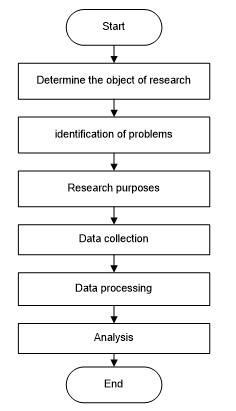
\includegraphics[scale=0.7]{figures/flowwc.PNG}
\caption{Flowchart research}
\label{labelgambar4}
\end{figure}

\section{Method Description}
Stages (groove strategies) the researchers used in the analysis of EEG data is as follows:

\begin{enumerate}
    \item Determine the object of research.
    \par
   Determine what object will be investigated in the research activity. Some things need to be understood to determine and construct an object of research in a research method, which relates to the purpose of research, besides that, each object of research and what criteria can be used as the purpose of the research that we do[19], in this study I had the opportunity to examine a drug user in the brain of the drug user and in this study I assessed brain waves by using EEG (Electrocardiograph) determination of brain waves to be explained here based on the amplitude of certain objects
   
    \item Identification of problems
    \par
   Problem identification is the process and result of problem recognition. In other words, problem identification is one of the research processes which is arguably the most important among other procedures. Research problems will determine the quality of research, in this step the researcher can find out more, can by conducting observations, reading the literature identifies one aspect that has been determined with the relevant environment (drug users) that is relevant.\cite{chappell2018constructing}
   
    \item Research purposes
    \par
    The purpose of this study was to obtain a formula for the results of research through the process of searching, discovering, developing, and testing surveys conducted.In this phase the researchers aimed to process the data. The purpose of this study could provide a basis for further developing research that builds evidence about brain waves of drug users\cite{chappell2018constructing}

    \item Data collection
    \par
    Data collection was conducted to obtain information required in achieving the goal of research being done. Before attending the study, the researchers usually have had a notion based on the theory that he used, each study had a data collection process that is different depending on the type of research that is being researched
    
    \item Data processing
    \par
 The image below is the process of processing data using Wavelet. the processed data is the data obtained from the EEG signal recording process, Bandpass Filter and ICA data after processing from Matlab. At this stage of data processing researchers conduct data processing on someone who is a drug user, at this stage researchers will also get the results of data processing in the form of amplitude..	
  
  \begin{figure}[h!]
\centering
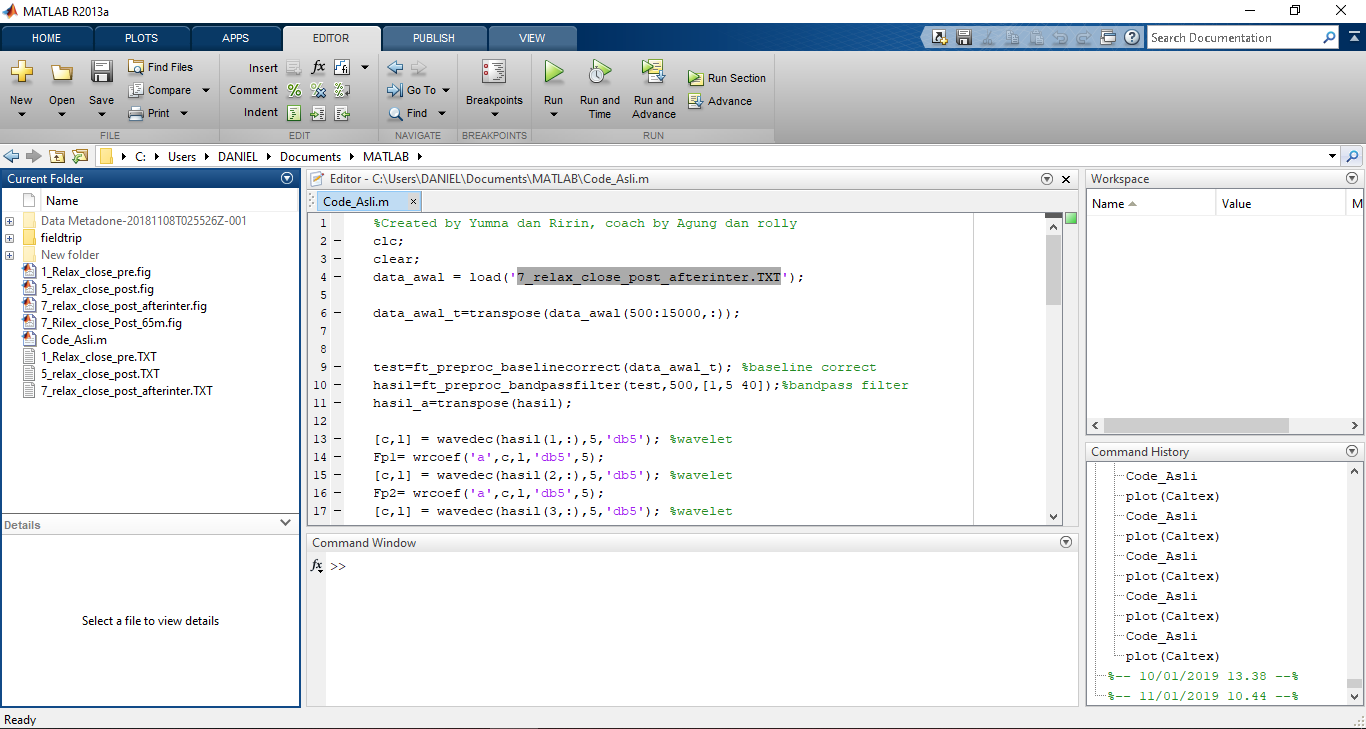
\includegraphics[scale=0.3]{figures/proses1.PNG}
\caption{Data Processing}
\label{labelgambar5}
\end{figure}
  
    \item results
    \par
    The results of processing the data researchers obtain information that has been processed beforehand and researchers get the results of brain waves of drug users.
    
\end{enumerate}

